\chapter{The Scratch Online Community}

%TODO: once settled with layout, make sure it does not use a full page just for this image
\begin{figure}
\centering
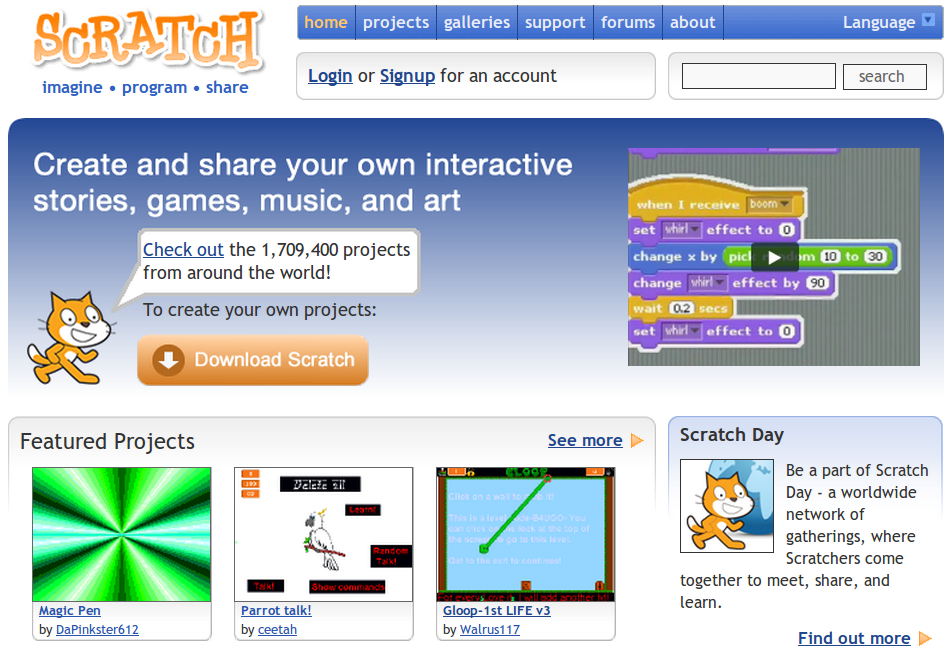
\includegraphics[width=3.25in]{figures/websitehomepage.png}
\caption{The home page of the Scratch website}
\label{fig:websitehomepage}
\end{figure}

The empirical setting for this work is the Scratch Online Community, a website (Figure~\ref{fig:websitehomepage}) I conceived and developed over the past four years, for this and other lines research.
The website allows anyone, especially young people between ages 8 and 16, to share their animated stories, interactive art, and video games. Participants use the Scratch programming environment to create or remix projects by putting together images, music and sounds with programming command blocks \citep{resnick_scratch:_2009}.
Projects range from interactive greeting cards, physics simulations, animations of popular songs to homemade video games, just to name a few.  

In my dissertation, I plan to document in detail the motivations that led to the design of the Scratch website as it is now and the different iterations that it went through as a result of internal and user-driven demands and participation patterns.
I will expand on the tight relationship between the technical capabilities of the website and the social dynamics that it supported or intended to support.
I will take a critical look at how the original goals of the community were or were not achieved and in what ways that happened. 
I will narrate scalability challenges with the technology and moderation of the community.
In the following two sections I provide a glimpse at this.

More broadly, I will try to tackle questions such as: How the culture of sharing was seeded and maintained in a public space? what were some important incidents that changed policies and/or architecutre? How did the architecture and management of the site influenced the culture of the site and how users helped shaped this? 
as it the design of the space or the work of users to create the culture?
 What were the lessons learned along the way by administrators? What kinds of learning outcomes were achieved?
To answer some of these questions, I will primarily rely on participant observation data, experiences collected during the three years and I will support of those arguments with descriptive statistics and case studies.


\section{Motivations}

From its inception \citep{monroy-hernandez_scratchr:_2007,monroy-hernandez_empowering_2008}, I set as the goal of the Scratch Online Community to give creators access to 
1) a \emph{network of peers} that functions as an audience and as potential collaborators and,
2) a \emph{repository} of inspirational creations and to that can be creatively appropriated by anyone.

More broadly, the Scratch Online Community was created with the idea of supporting a Community of Practice around Scratch where novices and experts would come together,  in the spirit of Papert's Samba school's metaphor \citep{papert_mindstorms_1980}.

Additionally, the idea of the Scratch Online Community was concieved under the umbrella of embodying the ethos of Participatory Culture of empowering people to become producers rather than just consumers of media.

Lastly, the Scratch Online Community was motivated to support the different iterative stages of the creative process \citep{resnick_sowing_2008}, namely:
Supporting creator's \emph{imagination} by giving access to a pool of inspirational projects and ideas; supporting \emph{creation} by allowing people to reuse and remix; supporting \emph{play} by letting people interact with others and their creations in the context of a community; supporting \emph{sharing} by allowing people to easily upload their creations to the platform; supporting \emph{reflection} by providing a space to receive comments and discussion forums for more in-depth discussions.

\section{Socio-technical infrastructure}
The Scratch website is broadly composed of the following components: 

1. A repository of projects and metadata. Projects can be downloaded by anyone, modified and reuploaded to the website as a remix. Each project has its own web page where it is displayed and where people can interact with it and other people.

2. A social network consisting of profile pages and unidirectional friendship connections. Profile pages list the friends, projects and favorited projects for each user along with his or her avatar image and the Country of origin (all self-reported data).

3. Social features for interacting with people's creation such as commenting, tagging, ``loving'', favoriting.

4. Galleries, which are pages where people can group projects and talk about them. It is important to note that galleries have been repurposed by the community as group spaces where people collaborate to create projects or use it as a space to talk to each other or play Role Playing Games.

5. Discussion forums where community members help each other with technical problems, find collaborators and talk about non-Scratch related activities that foster a sense of community on the website.

6. External services supported by APIs such as a website where people can link projects together or a Wiki where people can document their experiences with Scratch and the community.

The website runs on a hybrid model for moderation that combines user-driven moderation through flagging and appointed moderators workig in parallel with a full-time staff member and other part time ones that review the flags and make sure to keep the social dynamics as civil as possible. 
This model has allowed for scaling the community management at a low cost, however, a large part of the architecture and software development over the course of the three years have been put into mechanisms for preventing anti-social behavior.

Three years after its official release, the Scratch Online Community website I developed, handles more than ten million page views and 600 thousand people every month.
This web traffic is more than half of the page views of websites like newsweek.com \footnote{04/2011 data from http://www.quantcast.com/newsweek.com} and one third of a website like economist.com \footnote{04/2011 data from http://http://www.quantcast.com/economist.com}.
As of April of 2011, more than 1.7 million projects have been uploaded at an average of1 MB per project. 
Every second, the website receives up to 180 requests and it transfers 4MB.

In order to handle this level of activity, the website's architecture uses a caching engine for static content called Varnish and another one for dynamic content and database queries called Memcached. 
The website runs on a completely Free and Open Source software stack that includes Apache for its web server and MySQL for its database running on CentOS Linux. 
The web application is written using a PHP-based framework called CakePHP.
Additionally, the application supports external applications such as as a discussion forum, a user-driven wiki, a stats website and a couple of other websites that provide additional support to community members. 
These extra websites are supported via an API (Application Program Interface) that has allowed for escalability.
